\documentclass{beamer}
\mode<presentation>
\usetheme{CambridgeUS}
\usecolortheme{beaver}
\setbeamertemplate{caption}[numbered]

\usepackage[english]{babel}
\usepackage{graphicx}
\usepackage{subfigure}
\usepackage{url}
\usepackage[backend=bibtex, style=verbose]{biblatex}
\usepackage{multicol}
\bibliography{bibliography.bib}
\usepackage[noend]{algorithm,algpseudocode}


\title[LSTM: A Search Space Odysseys]{LSTM: A Search Space Odysseys}
\author[Mu\c sat Bogdan-Adrian]{Mu\c sat Bogdan-Adrian}
\date{February 2017}

\beamertemplatenavigationsymbolsempty
\graphicspath{{./images/}}

\begin{document}

\frame{\titlepage}

\begin{frame}
\frametitle{Recurrent Neural Networks - RNNs}
\center
\begin{itemize}
	\item Used to deal with sequential data, where there is a temporal dependence from a time instance to another
	\item Mathematically, they model a conditional distribution of the form \(P(x_t \lvert x_{t-1},..., x_2, x_1) \), where \(x_t\) is the current input at time \(t\)
	\item The output of a vanilla RNN cell at each time step is computed using the current input \(x_t\) and also the previous cell state \(h_{t-1}\)\footnote{Meant to encompass a summary of the past information} as:
	\[
		y_t = tanh(Ux_t + Wh_{t-1} + b),
	\]
	where \(U \in R^{M \times N}\), \(W \in R^{N \times N}\) are the shared parameter matrices for the RNN cells and \(b \in R^N\) is the bias
\end{itemize}
\end{frame}

\begin{frame}
\frametitle{Recurrent Neural Networks Unrolled}
\begin{figure}
	\subcapcentertrue
    \centering
    	\subfigure[RNN unrolled \footcite{Goodfellow-et-al-2016}] 
        {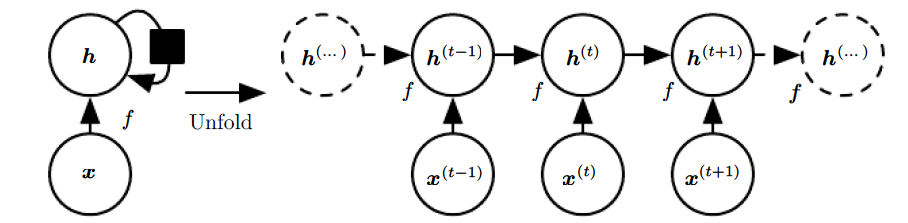
\includegraphics[width=1.0\textwidth]{rnn_unrolled.png}}
    \end{figure}   
\end{frame}

\end{document}